\documentclass[conference]{IEEEtran}

% -------------------------------------------------
% Pacchetti
% -------------------------------------------------
\usepackage[utf8]{inputenc}
\usepackage[T1]{fontenc}

\usepackage{amsmath,amssymb}
\usepackage{graphicx}
\usepackage{booktabs}
\usepackage{cite}
\usepackage{lipsum} % testo fittizio

% -------------------------------------------------
% Titolo
% -------------------------------------------------
\title{Data-Driven Basketball: Modelli Predittivi per l’Impatto Futuro dei Giocatori}

\author{
\IEEEauthorblockN{Simone Visconti}
\IEEEauthorblockA{
Università degli Studi di Salerno \\
s.visconti3@studenti.unisa.it
}

\and

\IEEEauthorblockN{Vincenzo Goffredo}
\IEEEauthorblockA{
Università degli Studi di Salerno \\
v.goffredo@studenti.unisa.it
}
}

% -------------------------------------------------
% Documento
% -------------------------------------------------
\begin{document}

\maketitle

% -------------------------------------------------
% Sezioni
% -------------------------------------------------
\section{Abstract}

In recent years, sports analytics has undergone a major revolution driven by the application of machine learning to optimize decision-making for coaches, scouts, and front offices. While the literature has heavily focused on team-level game outcome prediction or collective efficiency, accurately forecasting individual player trajectories on a seasonal scale remains a complex challenge. This short paper introduces a supervised machine learning framework to predict future offensive productivity—expressed as points per game (PPG) in the subsequent season—for National Basketball Association (NBA) players. The proposed dataset integrates biometric and anthropometric features (age, height, distance from the estimated athletic peak age of 27) with traditional in-game statistics, advanced metrics (e.g., True Shooting Percentage, Usage Rate, Net Rating), and historical career trends (lag features, a 3-season PPG slope, and career longevity). We implemented and compared several regression models: Linear Regression, Random Forest, Gradient Boosting, LightGBM and CatBoost. The evaluation on the 2023-24 validation set demonstrates that tree-based gradient-boosted models outperform traditional linear baselines. Specifically, CatBoost achieved the highest overall fit, yielding a Mean Absolute Error (MAE) of 2.06 PPG, a Root Mean Squared Error (RMSE) of 2.59 PPG, and a coefficient of determination $R^2$ of 0.849, while Random Forest achieved the lowest MAE of 2.05 PPG. The robust predictive results of the model show that combining age-related improvement and decline with past performance trends can be useful to estimate future player performance. This approach could therefore help professional franchises in decisions related to roster construction and player contract evaluation, even if further analyses would probably be needed to confirm the reliability of the model in different contexts.

\section{Introduction and Problem description}

\subsection{Background and Motivation}
In modern professional basketball, sports analytics has become a core predictive asset. The National Basketball Association (NBA) generates vast streams of high-dimensional, structured data, recording every action, possession, and biological metric of its athletes. 

Evaluating and predicting player performance is crucial for roster management, draft selection, contract negotiations, and salary cap optimization. Among all individual statistics, scoring productivity is arguably the most decisive factor. It directly influences game outcomes, defines player roles, and drives franchise commercial value, fan engagement, and media popularity. Consequently, modeling and predicting offensive output---specifically average points per game (PPG) and the outcome of a specific match---has emerged as a focal point in sports analytics. 

However, predicting individual performance trajectories over a seasonal horizon is a complex task. Unlike single-game forecasting, which is heavily influenced by immediate contextual factors (e.g., matchups, travel fatigue, home-court advantage), seasonal forecasting must capture long-term physiological changes, career development trends, and systemic shifts in team roles. 

\subsection{Problem Formulation}
We formulate our predictive task as a supervised regression problem aimed at forecasting the seasonal scoring productivity of NBA players. Specifically, the objective is to predict a player's average points per game (PPG) in the upcoming season based on their profile during the current season. Instead of relying on a single, isolated performance indicator, our approach structures each player's profile by combining multiple historical, performance-based, and physical attributes. 

The predictive models are trained on historical player-season data to learn the relationship between these multi-dimensional player profiles and their subsequent scoring outputs. To evaluate and validate model performance, the discrepancy between the predicted scoring averages and the actual results is measured using standard regression metrics, primarily Mean Absolute Error (MAE) and Root Mean Squared Error (RMSE). The final goal is to construct a generalizable framework that minimizes these prediction errors on unseen validation seasons.

To capture the diverse factors influencing a player's future scoring trajectory, the input features are organized into three primary domains:
\begin{itemize}
    \item \textbf{Biometric and Anthropometric Characteristics:} Features such as height, age, and a calculated distance from the theoretical athletic peak.
    \item \textbf{Current-Season Performance Metrics:} A combination of traditional statistics (e.g., minutes per game, rebounds, assists) and advanced efficiency ratings (e.g., True Shooting percentage, Usage Rate, Net Rating).
    \item \textbf{Historical Career Context (Lag Features \& Momentum):} Lagged metrics from prior seasons ($s-1$ and $s-2$), career longevity (number of seasons played), and a linear regression slope capturing the momentum of the player's scoring trajectory over the preceding three years.
\end{itemize}

\subsection{Challenges in Seasonal Performance Forecasting}
Predicting player performance from one season to the next presents unique statistical and biological challenges:
\begin{itemize}
    \item \textbf{The Aging Curve and Athletic Peak:} Athletic performance does not follow a linear trajectory. Physiological research indicates that professional basketball players generally reach their physical and athletic peak around the age of 27. Prior to this peak, players undergo physical maturation and skill development; after the peak, they experience progressive physical decline, which is often partially offset by increased tactical experience. Modeling this non-linear relationship is crucial for predicting long-term trajectories.
    \item \textbf{Mid-Season Transfers and Contextual Noise:} Professional players are frequently traded mid-season, resulting in multiple box-score entries with different teams. Averaging these statistics "raw" would ignore differences in playing time and game count, leading to data distortion. The data pipeline must apply weighted averages based on Games Played (GP) to maintain statistical integrity.
    \item \textbf{Injury and Outlier Filtering:} Severe injuries introduce massive noise into seasonal data. A player who suffers a season-ending injury in season $s+1$ will have an artificially low PPG that does not reflect their true performance capacity. Similarly, rookie players lack prior statistical history. The model must handle missing past data (\textit{NaN} values) through robust imputation (cloning current rookie values to simulate initial baselines) and filter out heavily injured players by enforcing minimum game and playing-time thresholds (e.g., minimum of 12 games and 120 minutes in the current season, and 20 games in the predicted season).
\end{itemize}

\subsection{Structure of the Paper}
The remainder of this paper is structured as follows:
\begin{itemize}
    \item \textbf{Section III (State of the Art and Related Works):} Reviews the existing literature on machine learning applications in sports analytics, analyzing the four foundational papers that guide this study.
    \item \textbf{Section IV (Proposed System):} Details the data engineering pipeline, data cleaning criteria, feature selection methods, and the mathematical formulations of the regression and ensemble models.
    \item \textbf{Section V (Experimental Results):} Presents the quantitative performance metrics (MAE, RMSE, $R^2$, and global accuracy) of all evaluated regressors on the validation dataset.
    \item \textbf{Section VI (Discussion):} Analyzes the results, explores feature importances, and discusses the practical implications of the findings for basketball scouts and front offices.
    \item \textbf{Section VII (Conclusions):} Summarizes the contributions of the project and outlines directions for future research.
\end{itemize}





\section{State of the Art and Related works}

The application of data mining and machine learning algorithms in sports analytics has expanded significantly, particularly in professional basketball. Existing research often falls into three main categories: team-level match outcome forecasting, team efficiency modeling, and individual player performance prediction. 

At the team level, predicting match outcomes is a well-studied problem. A study published in MDPI Applied Sciences~\cite{Panagiotis} developed a supervised machine learning framework to predict EuroLeague basketball game outcomes using team-level statistics. By comparing algorithms such as Logistic Regression, Support Vector Machines (SVM), Random Forests, and Naive Bayes, it has been demonstrated that SVM and Logistic Regression can capture linear and non-linear interactions in game-related metrics to predict wins and losses. This work emphasized the value of explainable artificial intelligence to provide actionable insights for coaches, identifying True Shooting percentage (TS\%), defensive rebounds, and steals as primary determinants of success.

In addition to game outcome prediction, modeling overall team efficiency has been explored to guide tactical decisions. Nousher~\cite{Nousher} compared Random Forest, Decision Tree, and Linear Regression models to evaluate basketball team efficiency and player efficiency ratings in the NBA. By leveraging historical team-level performance factors, their study highlighted that while ensemble models provide robust generalization, linear regression baselines can establish highly accurate and interpretable benchmarks when predicting overall team efficiency metrics. 

At the individual player level, the literature has explored both short-term and long-term performance forecasting. Chakrabarti~\cite{Chakrabarti} focused on short-term forecasting by predicting the number of points scored by a specific player in an upcoming individual game. Using Linear Regression, Neural Networks, Decision Trees, and Random Forests, the study introduced a Multiplicative Weight Update Algorithm (MWUA) to combine model predictions dynamically. Their findings indicated that while individual game performance is highly volatile, machine learning ensembles can successfully capture player scoring patterns.

On a seasonal scale, player-level performance and popularity have been modeled to support long-term franchise strategy. Nguyen et al.~\cite{Nguyen} investigated the application of machine learning and deep learning to predict both the long-term performance (measured through Win Shares) and the popularity (measured through All-Star game selection) of NBA players. Their comparative analysis showed that traditional machine learning algorithms, such as Random Forests, often outperform deep learning models on structured, relatively small sports datasets due to the risk of overfitting in deep networks. Crucially, their study identified scoring metrics as the most significant contributor to both performance evaluation and fan-driven popularity.

Despite these advancements, a gap remains in integrating biometric and physical characteristics with historical performance metrics to forecast player trajectory. While existing works focus either on short-term game-level points~\cite{Chakrabarti}, team-level outcomes~\cite{Panagiotis}, or general seasonal success indexes~\cite{Nguyen}, our proposed framework directly addresses the long-term prediction of season-long PPG. By combining biometric data (such as age, height, and distance from athletic peak) with historical performance lag features and multi-season momentum, this study bridges the gap between anthropometric evaluation and sports performance forecasting.

\section{Proposed Solution}


The proposed system consists of a machine learning pipeline written in Python. It aggregates player performance and biological data from multiple sources, processes and engineers features to capture player trajectories, and compares multiple regression models—including tree-based boosters—to forecast next-season scoring output. 

\subsection{Data Integration and Preprocessing}
The data is retrieved from three distinct CSV tables categorized by season: scoring statistics, biometric data, and traditional game statistics. The data integration pipeline executes the following steps:
\begin{itemize}
    \item \textbf{Merging:} For each season, the scoring and biometric tables are merged using a set of common keys (Player ID, Player Name, Team, and Season). Subsequently, the traditional box-score table is joined using Player ID, Season, and Team ID to extract additional statistics, such as steals (STL) and blocks (BLK), without creating duplicate features.
    \item \textbf{Unit Standardization:} Anthropometric indicators are standardized. Height, originally recorded in inches, is converted to centimeters ($Height = Height_{\text{inches}} \times 2.54$).
    \item \textbf{Traded Players Aggregation:} A common issue in sports databases is that players traded mid-season have multiple entries corresponding to their stints with different teams. To address this, the pipeline groups the merged dataset by Player ID and Season. Standard counting metrics (Games Played, Wins, Losses) are summed, while average game statistics (minutes per game, points per game, usage rate, etc.) are consolidated into a single row using a weighted average, where the weights are determined by the number of Games Played (GP) with each team during that season.
\end{itemize}

\subsection{Feature Engineering}
To capture both biological maturation and historical career trajectories, several advanced features are engineered:
\begin{itemize}
    \item \textbf{Biological Distance to Peak:} Following physiological findings that professional basketball players reach their physical and athletic peak at approximately 27 years of age, a Peak Age Distance feature is calculated as the absolute difference between the player's age and 27 ($PeakAgeDist = |Age - 27|$).
    \item \textbf{Historical Lag Features:} Using shift operations grouped by player, the pipeline introduces historical lag features from previous seasons ($s-1$ and $s-2$) for points per game, usage rate, and games played. To handle rookie players who lack past entries, their current-season statistics are cloned back to serve as historical baselines, preventing missing value issues.
    \item \textbf{Scoring Momentum:} To represent whether a player is improving, declining, or plateauing, a scoring momentum feature is calculated. This feature represents the slope of a linear regression fitted on the player's PPG over the preceding three seasons. To avoid data leakage, the regression uses a shifted window of past data, ensuring future values are never leaked.
    \item \textbf{Career Longevity:} A cumulative count of seasons played is computed for each player to represent their level of experience in the league.
\end{itemize}

\subsection{Data Cleaning and Filtering}
To ensure the models are trained on reliable data and to remove contextual noise, strict filtering criteria are applied:
\begin{itemize}
    \item \textbf{Minimum Playtime Filter:} Players who played fewer than 120 total minutes or fewer than 12 games in the current season are removed, as their statistics represent small-sample outliers.
    \item \textbf{Injury Filter in the Forecast Season:} To prevent major injuries from corrupting the target variable, players who played fewer than 20 games in the subsequent season ($s+1$) are excluded. This ensures the target ($NEXT\_PPG$) reflects a representative seasonal average rather than a partial, injury-shortened stint.
\end{itemize}

\subsection{Model Selection and Training Setup}
The processed dataset is split chronologically: all historical player-seasons up to the 2022-23 season are assigned to the training set, while the 2023-24 season is reserved for validation (predicting performance in the 2024-25 season). The framework implements and compares five regressors:
\begin{enumerate}
    \item \textbf{Linear Regression (Baseline):} A pipeline that applies standard scaling and a linear regressor, serving as a baseline.
    \item \textbf{Random Forest:} An ensemble of decision trees trained with default scikit-learn parameters.
    \item \textbf{Tuned Gradient Boosting Regressor:} A gradient booster configured with 200 estimators, a learning rate of 0.03, and a maximum tree depth of 4.
    \item \textbf{Tuned LightGBM Regressor:} A light gradient booster configured with 300 estimators, a learning rate of 0.03, a maximum depth of 3, and 20 leaves.
    \item \textbf{CatBoost Regressor:} An out-of-the-box CatBoost regressor designed to handle tabular features with high efficiency.
\end{enumerate}
The performance of these models is validated globally and tested on randomly selected individual players.

Both the Gradient Boosting Regressor and LightGBM were tuned utilizing GridSearchCV, which was employed to identify the optimal combination of hyperparameters from a predefined search grid.

\section{Results}

In this section, we present the quantitative evaluation of the five regression models on the validation set, which comprises player statistics from the 2023-24 season used to predict performance in the 2024-25 season. 

To contextualize the accuracy of the models, we first compute the standard deviation of the target variable ($NEXT\_PPG$) in the validation set, which stands at 6.66 PPG. This standard deviation serves as a baseline indicator of the inherent variability in scoring outputs across NBA players. 

The performance of each model was evaluated using four standard metrics: Mean Absolute Error (MAE), Root Mean Squared Error (RMSE), the coefficient of determination ($R^2$), and Global Accuracy (calculated as 100 minus the Weighted Mean Absolute Percentage Error, WMAPE). The results are summarized in Table~\ref{tab:results}.

\begin{table}[htbp]
\caption{Model Performance Evaluation on the 2023-24 Validation Set}
\label{tab:results}
\centering
\resizebox{\columnwidth}{!}{%
\begin{tabular}{lcccc}
\toprule
\textbf{Model} & \textbf{MAE (PPG)} & \textbf{RMSE (PPG)} & \textbf{R\textsuperscript{2}} & \textbf{Global Acc.} \\
\midrule
Linear Regression & 2.08 & 2.61 & 0.847 & 81.4\% \\
Random Forest & 2.05 & 2.62 & 0.845 & 81.6\% \\
Gradient Boosting (Tuned) & 2.06 & 2.64 & 0.843 & 81.6\% \\
LightGBM (Tuned) & 2.06 & 2.62 & 0.846 & 81.5\% \\
CatBoost & 2.06 & 2.59 & 0.849 & 81.5\% \\
\bottomrule
\end{tabular}%
}
\end{table}

\begin{figure}[htbp]
\centering
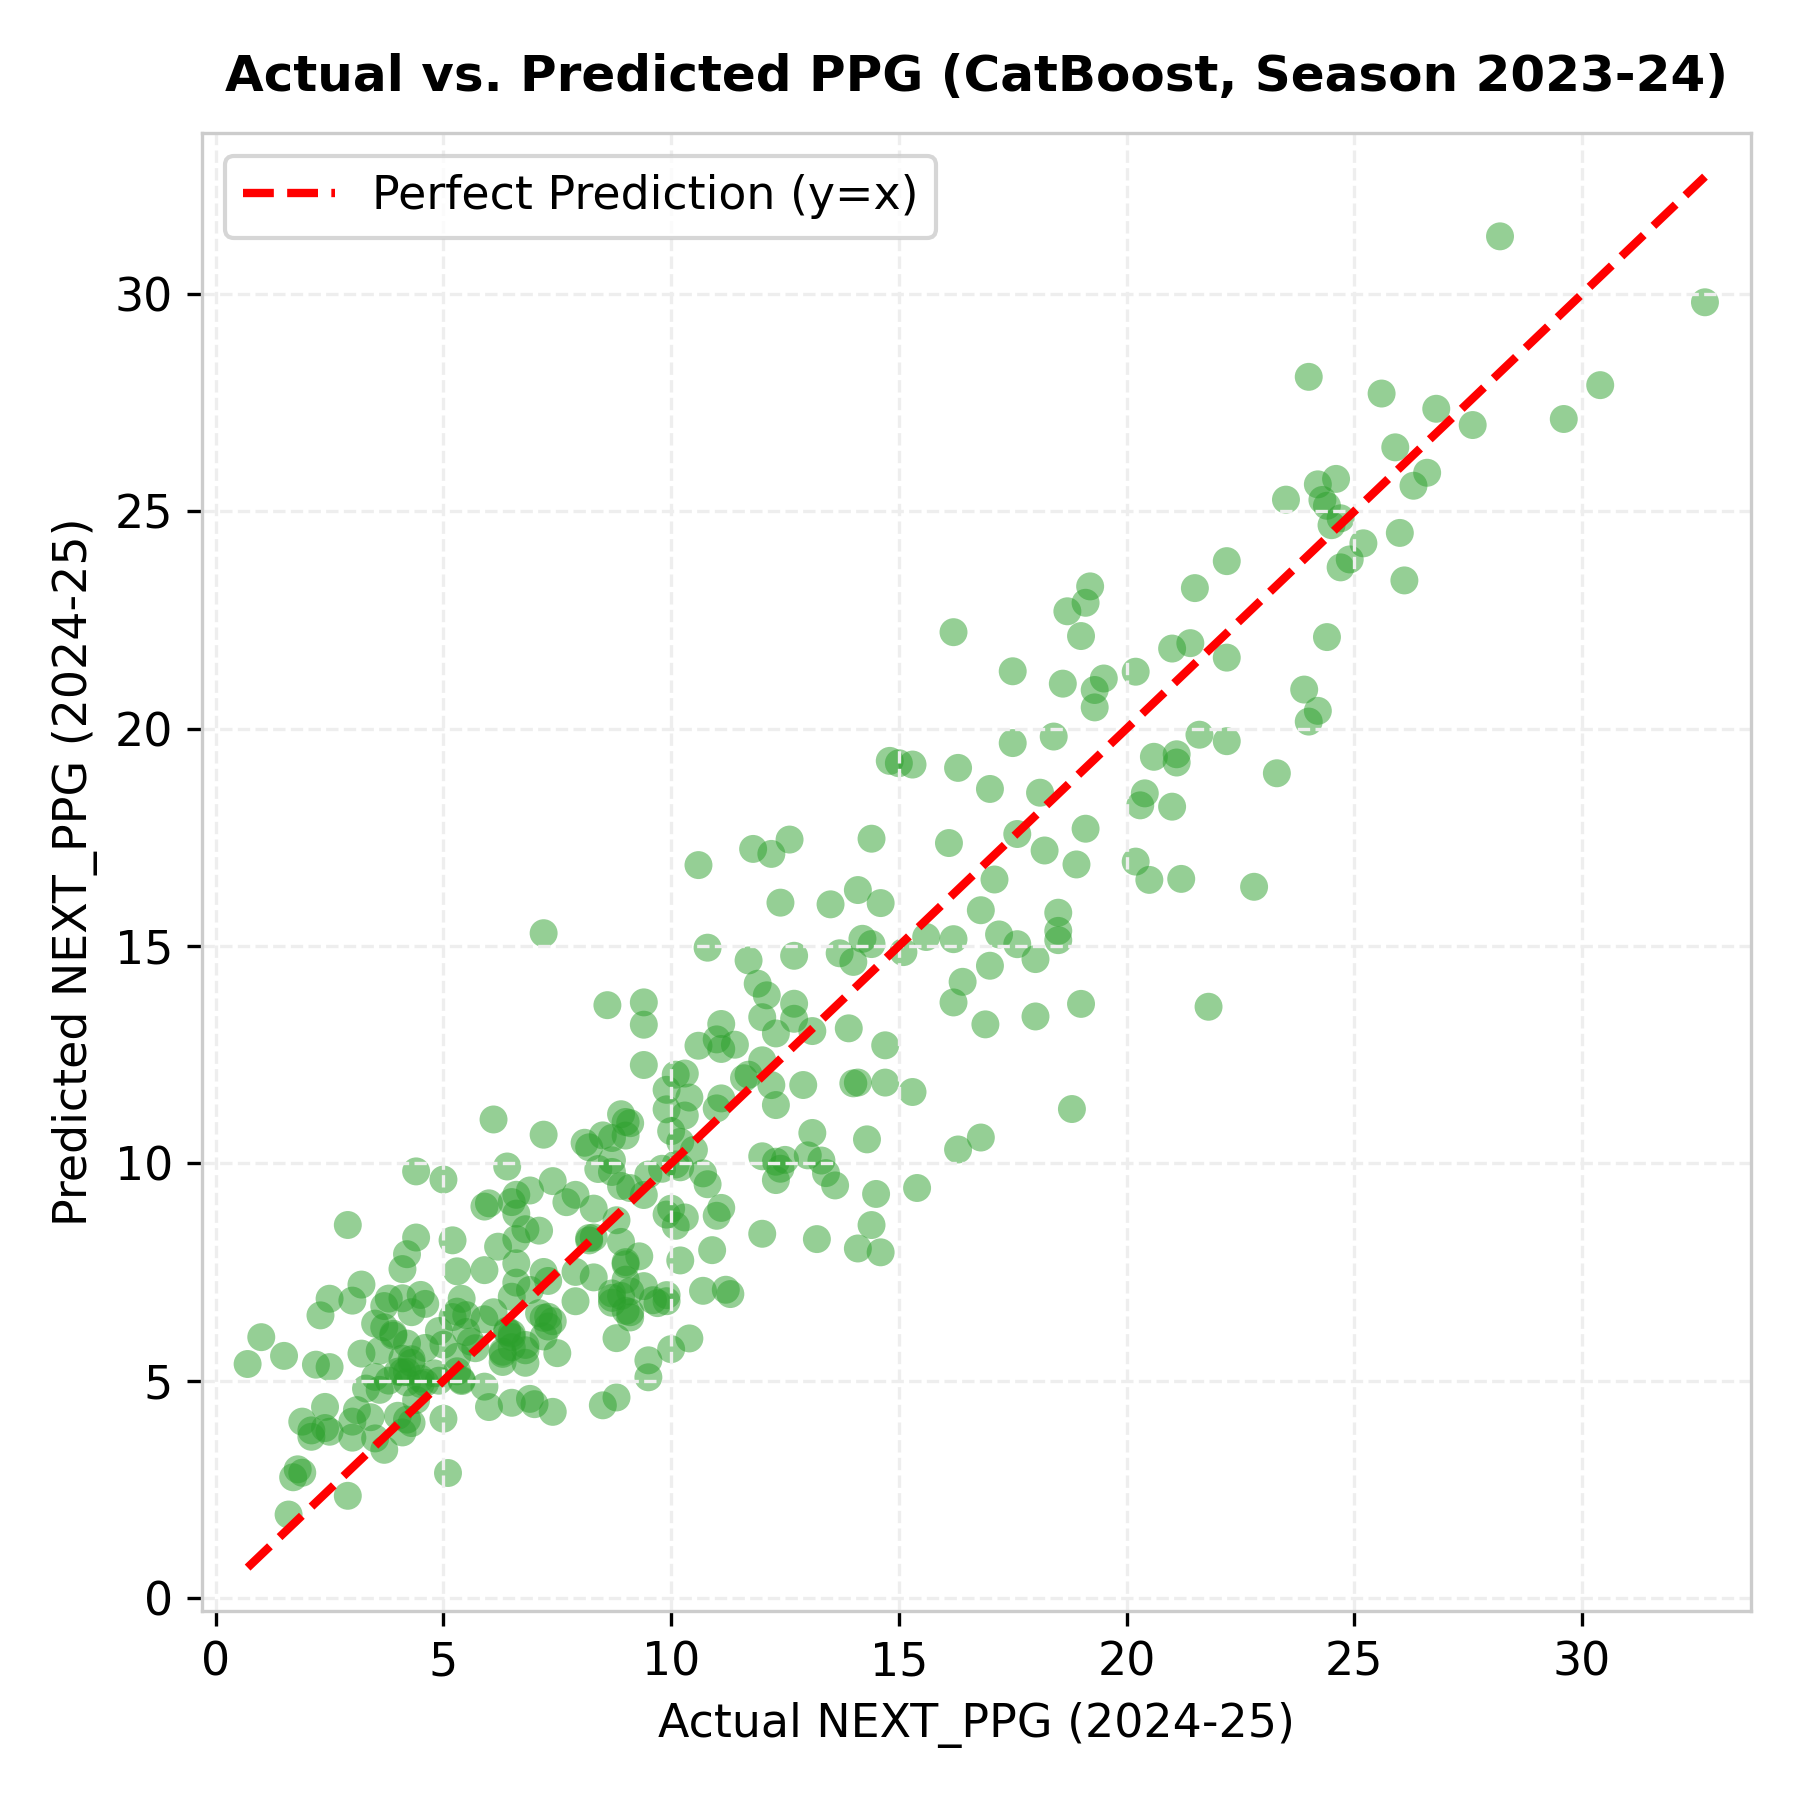
\includegraphics[width=\columnwidth]{actual_vs_predicted.png}
\caption{Actual versus predicted next-season PPG for CatBoost on the 2023-24 validation set. The dashed red diagonal line represents perfect predictions ($y=x$).}
\label{fig:actual_vs_predicted}
\end{figure}

The experimental results show that all five models exhibit strong predictive performance, with Mean Absolute Errors ranging between 2.05 and 2.08 PPG. This means that, on average, the models predict a player's next-season scoring average to within approximately two points of their actual outcome.

CatBoost achieved the highest overall fit, yielding the lowest RMSE of 2.59 PPG and the highest coefficient of determination ($R^2 = 0.849$), indicating that it explains 84.9\% of the variance in next-season player scoring. The Random Forest model achieved the lowest Mean Absolute Error (MAE = 2.05 PPG) and tied with Tuned Gradient Boosting for the highest Global Accuracy (81.6\%). Notably, the baseline Linear Regression model performed competitively, yielding an MAE of 2.08 PPG and an $R^2$ of 0.847. This strong baseline performance suggests that the engineered biometric, lag, and career momentum features are highly informative and linearly aligned with the target variable, reducing the marginal gain of complex non-linear models.


\section{Results discussion}

The experimental findings demonstrate that predicting individual seasonal scoring output is highly feasible when combining current-season performance, biometric parameters, and historical career trends. The fact that all models achieved a Mean Absolute Error of approximately 2.05--2.08 PPG against a target standard deviation of 6.66 PPG indicates that the engineered features successfully capture the underlying drivers of player scoring trajectories.

\subsection{Biometrics and the Physiological Aging Curve}
One of the key contributions of the proposed system is the integration of biometric data, specifically age and the biological distance to the athletic peak (\textit{PEAK\_AGE\_DIST}), which is established at 27 years. In sports biology, age-related performance curves are highly non-linear. By providing the model with both chronological age and the absolute distance to the peak age, tree-based models can segment players into distinct developmental phases:
\begin{itemize}
    \item \textbf{Maturation Phase:} Younger players (e.g., aged 19--24) who show high usage and positive momentum are likely to see an increase in PPG as they approach their physical peak.
    \item \textbf{Peak Phase:} Players near 27 years of age exhibit stable performance with high durability, sustaining high scoring outputs.
    \item \textbf{Decline Phase:} Older players (e.g., aged 32+) who score at a high level are expected to experience a gradual physical decline. The model uses the age features to scale down their predicted future PPG, capturing the physical constraints of aging.
\end{itemize}
This biometric integration enables the model to distinguish between two players who share identical current-season statistics but have completely different career trajectories due to their biological states.

\begin{figure}[htbp]
\centering
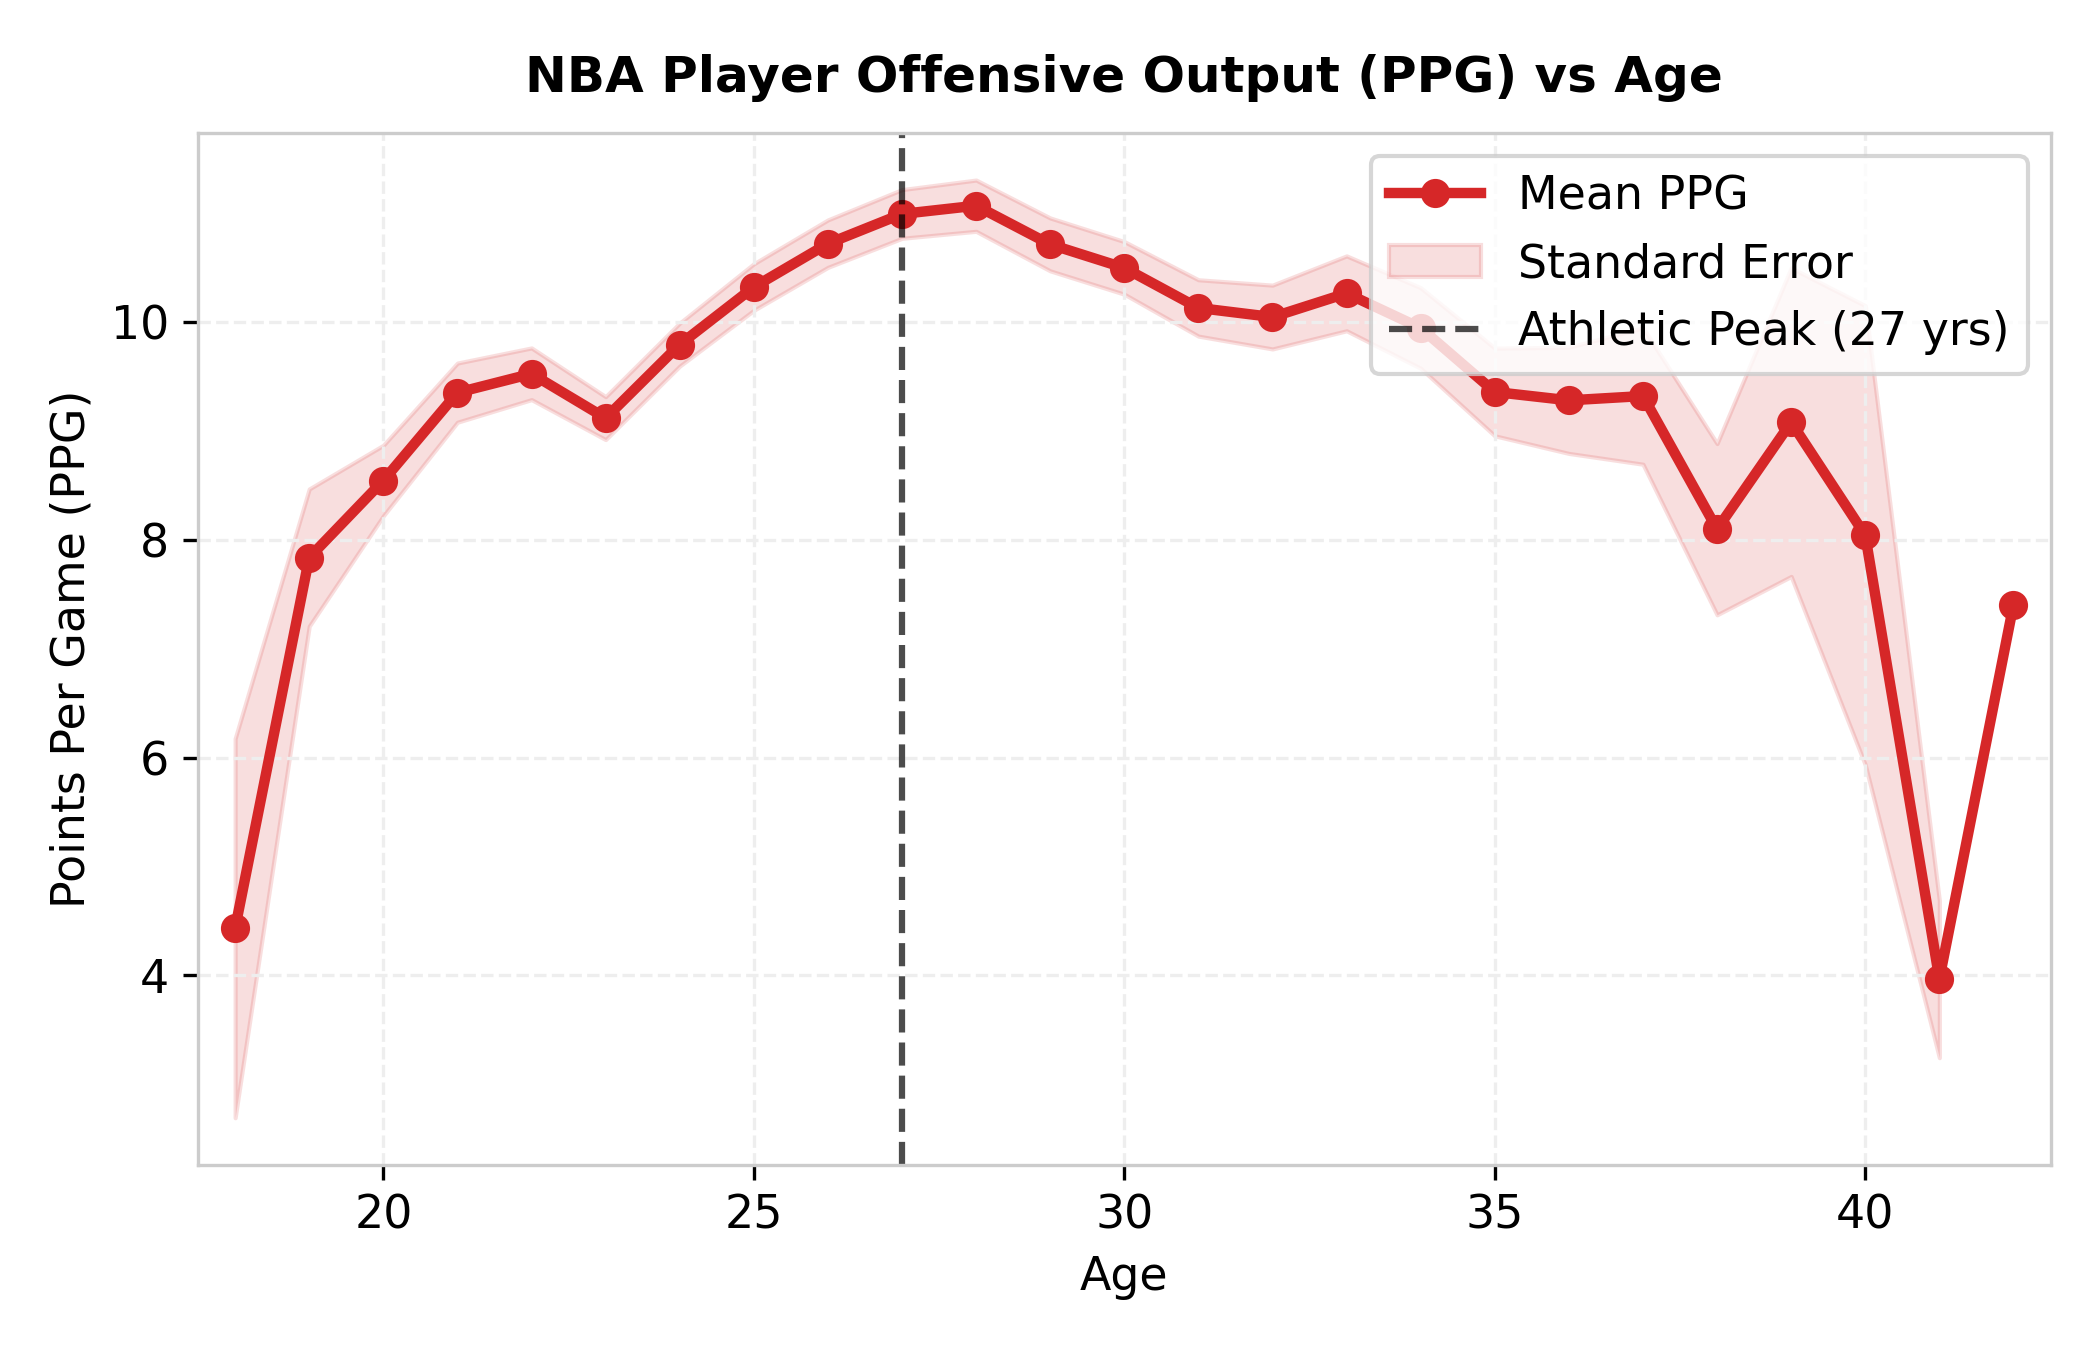
\includegraphics[width=\columnwidth]{aging_curve.png}
\caption{NBA players' average PPG as a function of age across the entire dataset. The dashed black line represents the estimated athletic peak age of 27.}
\label{fig:aging_curve}
\end{figure}

\subsection{Impact of Career Momentum and Lag Features}
The inclusion of career momentum (\textit{PPG\_MOMENTUM}) and lag features provides temporal continuity that a single-season model would lack. The momentum feature, representing the three-year slope of scoring averages, acts as a proxy for player trajectory. A positive slope indicates an athlete who is expanding their role or improving their shooting efficiency, which correlates with future increases. Conversely, a negative slope indicates a persistent decline, helping the model correct predictions downward. 

Furthermore, historical lag features like \textit{PREV\_PPG} and \textit{PREV\_PPG\_2} act as regularizers. They prevent the model from overreacting to single-season outliers, such as a player having an exceptional shooting year or a temporary drop in production due to minor injuries or system adjustments.

\subsection{Linear vs. Non-Linear Modeling Trade-offs}
A notable finding is the highly competitive performance of the baseline Linear Regression model ($R^2 = 0.847$), which performs only slightly below CatBoost ($R^2 = 0.849$). This suggests that the relationship between a player's current-season statistics (such as usage rate, playing time, and scoring) and their future output is predominantly linear. 

However, tree-based models like CatBoost and Random Forest still yield marginal improvements because they can capture complex interaction effects that a standard linear model ignores. For example, a high usage rate (\textit{USG\%}) typically leads to higher scoring, but this relationship is mediated by minutes played (\textit{MPG}) and shooting efficiency (\textit{TS\%}). Tree-based models naturally partition the feature space to model these synergistic interactions (e.g., high usage is only sustainable and productive when accompanied by high true shooting efficiency).

\begin{figure}[htbp]
\centering
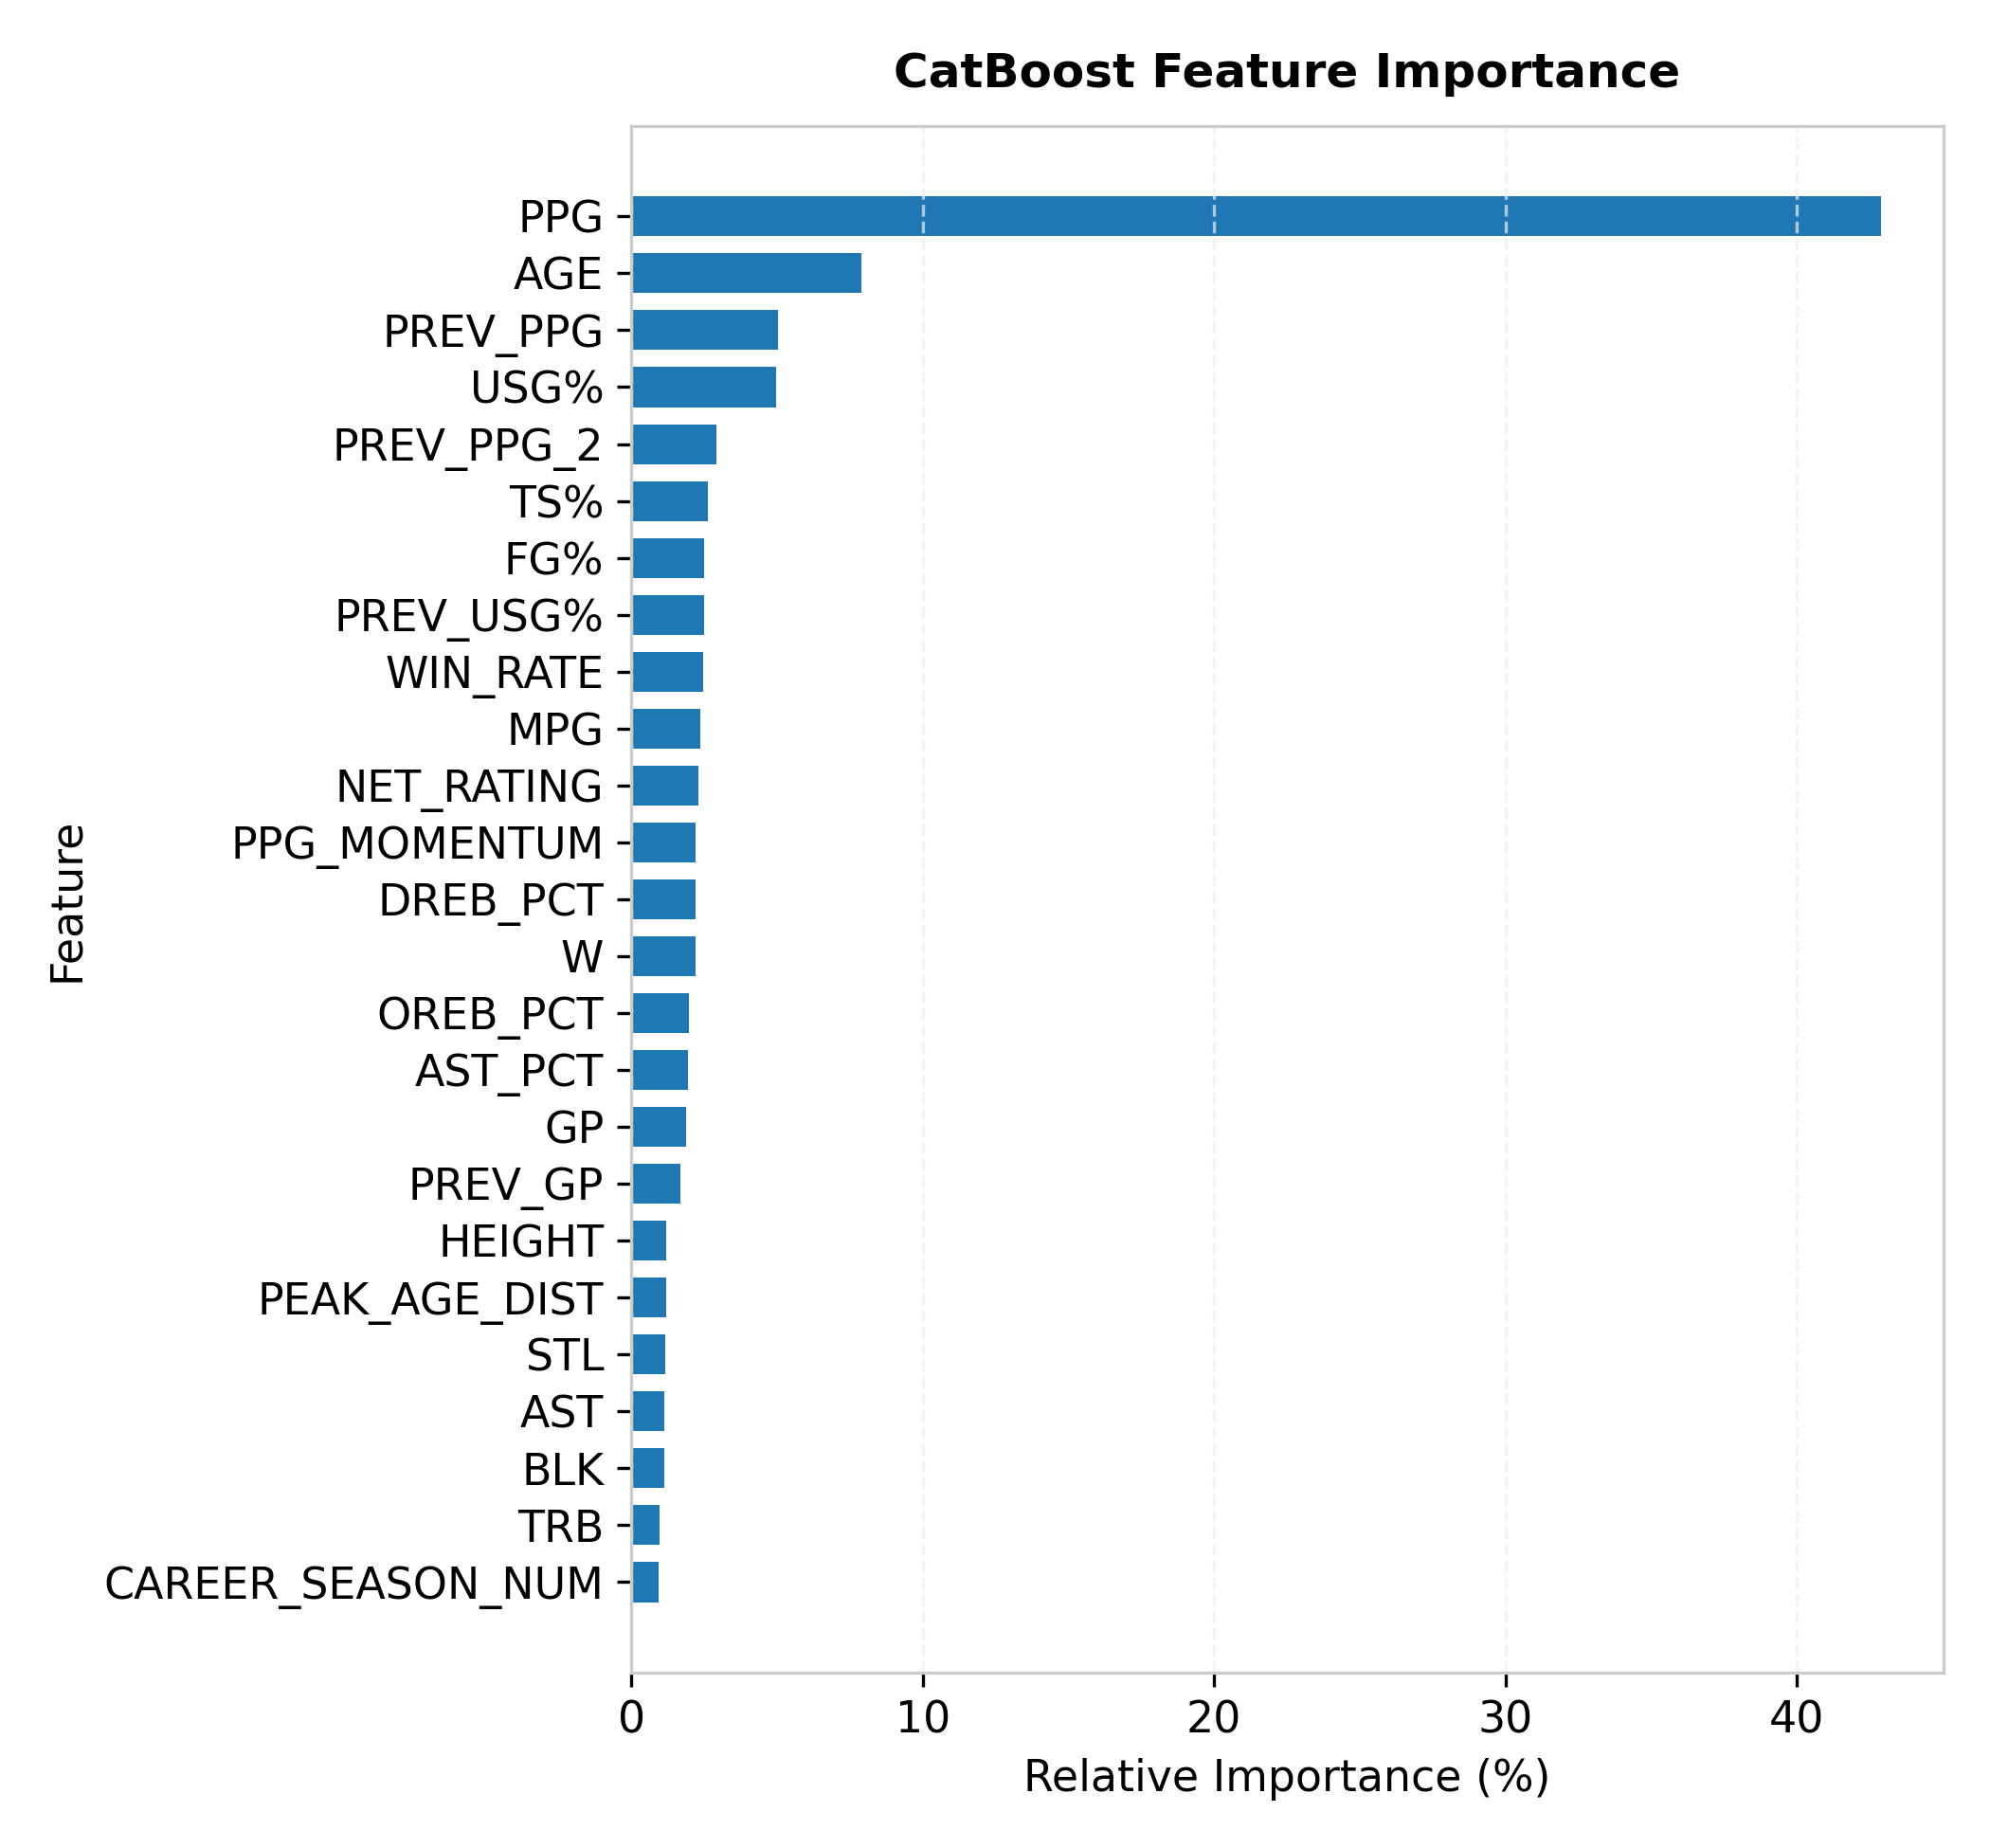
\includegraphics[width=\columnwidth]{feature_importance.png}
\caption{Relative feature importances of the CatBoost regressor, highlighting the significance of current-season points, minutes played, and historical lag statistics.}
\label{fig:feature_importance}
\end{figure}

\subsection{Limitations}
While the proposed framework demonstrates robust predictive accuracy, several limitations must be acknowledged. The current model relies entirely on individual box-score metrics and biometrics, thereby ignoring broader team-level contextual shifts. Factors such as changes in coaching staff, team tactical systems, or roster modifications—such as a star teammate leaving or joining, which can drastically alter a player's usage and role—are not captured. Future work could address these limitations by integrating team-level variables or graph-based teammate representations to capture these complex contextual dynamics.


\section{Conclusions}
In this paper, we presented a supervised machine learning framework to forecast individual player scoring trajectories in the NBA on a seasonal horizon. By combining physical and biometric data with historical game performance and career momentum, the proposed pipeline models both the biological development of athletes and their tactical roles. 

Our experimental evaluation compared five regression models on the 2023-24 validation set. The results demonstrate high predictive performance, with all models achieving a Mean Absolute Error of approximately two points per game. CatBoost yielded the highest overall fit, explaining 84.9\% of the variance in next-season scoring ($R^2 = 0.849$, $RMSE = 2.59$ PPG), while Random Forest achieved the lowest absolute error ($MAE = 2.05$ PPG). The competitive performance of the standard Linear Regression baseline ($R^2 = 0.847$) indicates that the engineered biometric features (such as distance to peak athletic age) and trajectory indicators (such as multi-season scoring momentum) are strongly aligned with future performance. 

Ultimately, this study confirms that integrating physiological aging parameters with historical performance metrics provides a reliable framework for player trajectory forecasting.

% -------------------------------------------------
% Bibliografia
% -------------------------------------------------
\bibliographystyle{IEEEtran}

\begin{thebibliography}{00}

\bibitem{Nguyen}
N.~H. Nguyen, D.~T.~A. Nguyen, B.~Ma, and J.~Hu,
``The application of machine learning and deep learning in sport: predicting NBA players' performance and popularity,''
\textit{Journal of Information and Telecommunication}, vol. 6, no. 2, pp. 217--235, 2022,
DOI: 10.1080/24751839.2021.1977066.

\bibitem{Chakrabarti}
A.~Chakrabarti,
``Leveraging Machine Learning for Predicting NBA Player Performance,''
\textit{National High School Journal of Science}, 2025.

\bibitem{Panagiotis}
P.~F. Foteinakis, C.~Kokkotis, G.~Karamousalidis, A.~Avloniti, S.~Pavlidou, N.~Zaras, T.~Stampoulis, D.~Pantazis, P.~Aggelakis, D.~Balampanos, J.~Liu, K.~Laparidis, and A.~Chatzinikolaou,
``From Data to Decisions: Using Explainable Machine Learning to Predict EuroLeague Basketball Outcomes,''
\textit{Applied Sciences}, vol. 15, no. 23, p. 12401, 2025.

\bibitem{Nousher}
K.~Nousher,
``Basketball Performance Prediction Models and Team Efficiency Factors,''
MSc Research Project, School of Computing, National College of Ireland, 2023.

\end{thebibliography}

\end{document}